% Hlavicka pro protokoly z fyzikalniho praktika.
% Verze pro: LaTeX
% Verze hlavicky: 22. 2. 2007
% Autor: Ustav fyziky kondenzovanych latek
% Ke stazeni: www.physics.muni.cz/ufkl/Vyuka/
% Licence: volne k pouziti, nejlepe k vcasnemu odevzdani protokolu z Vaseho mereni.


\documentclass[czech,11pt,a4paper]{article}
\usepackage[T1]{fontenc}
\usepackage{graphicx}
\usepackage{mathtools}
\usepackage{amssymb}
\usepackage{amsthm}
\usepackage{thmtools}
\usepackage{xcolor}
\usepackage{nameref}
\usepackage{babel}
\usepackage{hyperref}


%%% Nemente:
\usepackage[margin=2cm]{geometry}
\newtoks\jmenopraktika \newtoks\jmeno \newtoks\datum
\newtoks\obor \newtoks\skupina \newtoks\rocnik \newtoks\semestr
\newtoks\cisloulohy \newtoks\jmenoulohy
\newtoks\tlak \newtoks\teplota \newtoks\vlhkost
%%% Nemente - konec.


%%%%%%%%%%% Doplnte pozadovane polozky:

\jmenopraktika={Fyzikální praktikum 1}  % nahradte jmenem vaseho predmetu
\jmeno={Teodor Duraković}            % nahradte jmenem mericiho
\datum={20.~března 2024}        % nahradte datem mereni ulohy
\obor={F}                     % nahradte zkratkou vami studovaneho oboru
\skupina={St 8:00}            % nahradte dobou vyuky vasi seminarni skupiny
\rocnik={I}                  % nahradte rocnikem, ve kterem studujete
\semestr={II}                 % nahradte semestrem, ve kterem studujete

\cisloulohy={7}               % nahradte cislem merene ulohy
\jmenoulohy={Měření Poissonovy konstanty vzduchu} % nahradte jmenem merene ulohy

\tlak={99399}                   % nahradte tlakem pri mereni (v hPa)
\teplota={20.6}               % nahradte teplotou pri mereni (ve stupnich Celsia)
\vlhkost={36.9}               % nahradte vlhkosti vzduchu pri mereni (v %)

%%%%%%%%%%% Konec pozadovanych polozek.


%%%%%%%%%%% Uzitecne balicky:

%%%%%% Zamezeni parchantu:
\widowpenalty 10000 \clubpenalty 10000 \displaywidowpenalty 10000
%%%%%% Parametry pro moznost vsazeni vetsiho poctu obrazku na stranku
\setcounter{topnumber}{3}	  % max. pocet floatu nahore (specifikace t)
\setcounter{bottomnumber}{3}	  % max. pocet floatu dole (specifikace b)
\setcounter{totalnumber}{6}	  % max. pocet floatu na strance celkem
\renewcommand\topfraction{0.9}	  % max podil stranky pro floaty nahore
\renewcommand\bottomfraction{0.9} % max podil stranky pro floaty dole
\renewcommand\textfraction{0.1}	  % min podil stranky, ktery musi obsahovat text
\intextsep=8mm \textfloatsep=8mm  %\intextsep pro ulozeni [h] floatu a \textfloatsep pro [b] or [t]

% Tecky za cisly sekci:
\renewcommand{\thesection}{\arabic{section}.}
\renewcommand{\thesubsection}{\thesection\arabic{subsection}.}
% Jednopismenna mezera mezi cislem a nazvem kapitoly:
\makeatletter \def\@seccntformat#1{\csname the#1\endcsname\hspace{1ex}} \makeatother


%%%%%%%%%%%%%%%%%%%%%%%%%%%%%%%%%%%%%%%%%%%%%%%%%%%%%%%%%%%%%%%%%%%%%%%%%%%%%%%
%%%%%%%%%%%%%%%%%%%%%%%%%%%%%%%%%%%%%%%%%%%%%%%%%%%%%%%%%%%%%%%%%%%%%%%%%%%%%%%
% Zacatek dokumentu
%%%%%%%%%%%%%%%%%%%%%%%%%%%%%%%%%%%%%%%%%%%%%%%%%%%%%%%%%%%%%%%%%%%%%%%%%%%%%%%
%%%%%%%%%%%%%%%%%%%%%%%%%%%%%%%%%%%%%%%%%%%%%%%%%%%%%%%%%%%%%%%%%%%%%%%%%%%%%%%

\begin{document}
	
	%%%%%%%%%%%%%%%%%%%%%%%%%%%%%%%%%%%%%%%%%%%%%%%%%%%%%%%%%%%%%%%%%%%%%%%%%%%%%%%
	% Nemente:
	%%%%%%%%%%%%%%%%%%%%%%%%%%%%%%%%%%%%%%%%%%%%%%%%%%%%%%%%%%%%%%%%%%%%%%%%%%%%%%%
	\thispagestyle{empty}
	
	{
		\begin{center}
			\sf 
			{\Large Ústav fyzikální elektroniky Přírodovědecké fakulty Masarykovy univerzity} \\
			\bigskip
			{\huge \bfseries FYZIKÁLNÍ PRAKTIKUM} \\
			\bigskip
			{\Large \the\jmenopraktika}
		\end{center}
		
		\bigskip
		
		\sf
		\noindent
		\setlength{\arrayrulewidth}{1pt}
		\begin{tabular*}{\textwidth}{@{\extracolsep{\fill}} l l}
			\large {\bfseries Zpracoval:}  \the\jmeno & \large  {\bfseries Naměřeno:} \the\datum\\[2mm]
			\large  {\bfseries Obor:} \the\obor  \hspace{40mm}  {\bfseries Skupina:} \the\skupina %
			%{\bfseries Ročník:} \the\rocnik \hspace{5mm} {\bfseries Semestr:} \the\semestr  
			&\large {\bfseries Testováno:}\\
			\\
			\hline
		\end{tabular*}
	}
	
	\bigskip
	
	{
		\sf
		\noindent \begin{tabular}{p{3cm} p{0.7\textwidth}}
			\Large  Úloha č. {\bfseries \the\cisloulohy:} \par
			\smallskip
			$T=\the\teplota$~$^\circ$C \par
			$p=\the\tlak$~Pa    \par
			$\varphi=\the\vlhkost$~\%
			&\Large \bfseries \the\jmenoulohy  \\[2mm]
		\end{tabular}
	}
	
	\vskip1cm
	
	%%%%%%%%%%%%%%%%%%%%%%%%%%%%%%%%%%%%%%%%%%%%%%%%%%%%%%%%%%%%%%%%%%%%%%%%%%%%%%%
	% konec Nemente.
	%%%%%%%%%%%%%%%%%%%%%%%%%%%%%%%%%%%%%%%%%%%%%%%%%%%%%%%%%%%%%%%%%%%%%%%%%%%%%%%
	
	%%%%%%%%%%%%%%%%%%%%%%%%%%%%%%%%%%%%%%%%%%%%%%%%%%%%%%%%%%%%%%%%%%%%%%%%%%%%%%%
	%%%%%%%%%%%%%%%%%%%%%%%%%%%%%%%%%%%%%%%%%%%%%%%%%%%%%%%%%%%%%%%%%%%%%%%%%%%%%%%
	% Zacatek textu vlastniho protokolu
	%%%%%%%%%%%%%%%%%%%%%%%%%%%%%%%%%%%%%%%%%%%%%%%%%%%%%%%%%%%%%%%%%%%%%%%%%%%%%%%
	%%%%%%%%%%%%%%%%%%%%%%%%%%%%%%%%%%%%%%%%%%%%%%%%%%%%%%%%%%%%%%%%%%%%%%%%%%%%%%%
	
	
	\section{Zadání}
	Zjistit Poissonovu konstantu:
	1) Clément-Desormesovou metodou pomocí diferenciálního tlakového čidla a U trubice
	2) Prostřednictvím měření maxim vlnových délek stojatého vlnění v Kundtově trubici.
	
	\section{Postup}
	Poissonova konstanta, označovaná $\kappa$, je konstantou vyskytující se ve vztahu pro adiabatický děj
	v~ideálním plynu
	\begin{equation}
		pV^{\kappa} = konst.
	\end{equation}
	Poissonovu konstantu můžeme určit jako $\kappa = \frac{C_p}{C_v} $, kde $C_p$ je molární tepelná kapacita při stálém tlaku a $C_V$ molární tepelná kapacita při stálém objemu. Tyto hodnoty jsou závislé na počtu atomů tvořících vyšetřovaný plyn, tepelná kapacita se totiž odvíjí od toho, kolika způsoby může plyn tepelnou energii absorbovat a manifestovat, resp. kolika stupňů volnosti molekula daného plynu disponuje. Jelikož je námi zkoumaný vzduch tvořen z převážně dvouatomových molekul, budeme se soustředit právě na dvouatomový plyn. U vzduchu se za laboratorní teploty projevuje pět stupňů volnosti: tři translační a~dva rotační. Vibrace se projevuje až u vyšších teplot. Pro zkoumaný plyn dle ekvipartičního teorému tedy platí:

	\begin{gather}
			C_V = \frac {\partial E}{\partial T}_V = \frac{N \partial \langle \varepsilon \rangle}{\partial T}_V = N \frac{d \frac{5}{2}kT}{dT} = \frac 5 2 Nk = \frac 5 2 nR \\
		C_p = C_V + nR = \frac 7 2 nR
		\end{gather}
		kde $N$ je počet částic, $n$ látkové množství plynu, $R$ univerzální plynová konstanta a $\langle \varepsilon \rangle $ je střední hodnota energie (v našem případě translační a rotační) jedné částice.
		Pro Poissonovu konstantu platí:
		\begin{equation}
			\kappa = 1.4
		\end{equation}
		
		\subsection{Clément-Desormesova metoda}
			Aparatura se sestává z velké nádoby, malého napouštěcího a velkých vypouštěcích ventilů a tlakoměrů. Nádoba se tlakuje	ruční pumpičkou přes malý oddělovací ventil. Vypouštění plynu z nádoby lze provést otevřením
			velkého ručního ventilu. Nádoba je opatřena dvěma tlakoměry, které měří přetlak vzhledem k okolní atmosféře – U trubicí a průmyslovým diferenciálním tlakovým čidlem. Postupujeme následovně:\\
			0.	Před každým měřením za otevření velkého ventilu poznamenáme proud na ampérmetru napojeném na diferenciální tlakové čidlo. Tato hodnota nám stanovuje proud $I_0$, tedy proud při nulovém rozdílu tlaků.
			1.	Otevřeme malý ventil a ruční pumpičkou zvýšíme tlak v nádobě. Ventil uzavřeme a systém necháme dosáhnout termodynamické rovnováhy s okolím (plyn se bude izochoricky ochlazovat, proto budeme pozorovat pokles tlaku).\\
			2.	Po ustálení tlaku jej odečteme z měřících přístrojů, poznamenáme hodnotu $p_1$.\\
			3.	Rychlým otočením velkého ventilu uskutečníme adiabatickou expanzi vzduchu. Ventil okamžitě uzavřeme, izobarický ohřev by do měření přinesl systematickou chybu. S uzavřeným ventilem se systém zahřívá izochoricky, sledujeme růst tlaku. Po dosažení termodynamické rovnováhy s okolím pozorujeme ustálení tlaku. Odečteme z přístrojů hodnotu $p_2$.\\
			
		\subsection{Měření Poissonovy konstanty z rychlosti zvuku v plynu}
		V Kundtově trubici měříme polohy maxim pro různé vlnové délky. Rozdíl poloh sousedních maxim $d$ se rovná polovině vlnové délky, jsme tedy schopni určit vlnovou délku. Pro rychlost zvuku $c$ bude platit vztah:
		\begin{equation}
			c = 2 \overline{d}f,
		\end{equation}
		kde $f$ je nastavená frekvence.
		Pro výpočet $d$ použijeme metodu nejmenších čtverců. Pro každou frekvenci zvlášť do grafu vyneseme polohu každého naměřeného maxima jako funkci jeho pořadí a závislost	proložíme lineární funkcí.
		Pro ideální plyn platí pro rychlost vztah
		\begin{equation}
			c = \sqrt{\frac{\kappa p}{\rho}},
		\end{equation}
		pro výpočet Poissonovy konstanty tudíž platí
		\begin{equation}
			\kappa = \frac{c^2 \rho}{p} = \frac {{(2\overline{d}f)}^2 \rho}p
		\end{equation}
		\subsection{Údaje používaných přístrojů}
		\begin{center}
			\begin{tabular}{|l|l|c|}
				\hline
				Název přístroje & typ přístroje           & standardní nejistota   \\ \hline \hline
				Metex 3292      & ampérmetr  (výstup diferenciálního tlakoměru)   &   $0.007\%$     \\ \hline
			    (voda v U trubici)  & tlakoměr               & $ 0.3 $ mm \\ \hline
				  & Svinovací metr (v Kundtově trubici)   &$ 0.3 $ mm\\ \hline
			\end{tabular}
		\end{center}
	
	\newpage
	\section{Měření}
	\subsection{Clément-Desormesova metoda}
	Při měření získáváme následující údaje:
	
	
	\begin{center}
		\begin{tabular}{|l|c|c|c|}
		\hline
		 &$h_1$  [mm]& $h_2$ [mm]  & $\kappa$ \\ \hline
		1&238 & 60  & 1.34                  \\ \hline
		2&235 & 60  & 1.34                  \\ \hline
		3&244 & 61  & 1.33                  \\ \hline
		4&420 & 107 & 1.34                  \\ \hline
		5&332 & 105 & 1.46                  \\ \hline
		6&340 & 90  & 1.36                  \\ \hline
		7&165 & 44  & 1.36                  \\ \hline
		8&248 & 70  & 1.39                  \\ \hline
		9&280 & 87  & 1.45                  \\ \hline
		10&243 & 64  & 1.36                  \\ \hline  \hline
		$\overline{x}$&274.5 & 74.8  & 1.37                  \\ \hline
		
		
	\end{tabular}
	\begin{tabular}{|l|c|c|c|c|}
		\hline
		& \multicolumn{1}{l|}{$I_0$ {[}mA{]}} & \multicolumn{1}{l|}{$I_1$ {[}mA{]}} & \multicolumn{1}{l|}{$I_2${[}mA{]}} & \multicolumn{1}{l|}{$\kappa$} \\ \hline
		1  & 4.0331                           & 11.473                          & 5.8868                          & 1.33                       \\ \hline
		2  & 4.0382                           & 11.396                          & 5.9884                          & 1.36                       \\ \hline
		3  & 4.0423                           & 11.705                          & 5.9634                          & 1.33                       \\ \hline
		4  & 4.0445                           & 17.220                           & 7.4407                          & 1.35                       \\ \hline
		5  & 4.0510                            & 14.466                          & 7.3916                          & 1.47                       \\ \hline
		6  & 4.0516                           & 14.690                         & 6.8243                          & 1.35                       \\ \hline
		7  & 4.0525                           & 9.2140                           & 5.4430                           & 1.37                       \\ \hline
		8  & 4.0518                           & 11.830                           & 6.2390                           & 1.39                       \\ \hline
		9  & 4.0531                           & 12.833                          & 6.4740                           & 1.38                       \\ \hline
		10 & 4.0547                           & 11.640                           & 6.0623                          & 1.35                       \\ \hline \hline
		$\overline{x}$  & \multicolumn{1}{c|}{4.05}        & \multicolumn{1}{c|}{12.65}      & \multicolumn{1}{c|}{6.37}       & \multicolumn{1}{c|}{1.37}  \\ \hline
	\end{tabular}
	\end{center}
	
	\subsection{Zpracování měření}
	Vztahem \begin{equation}
		\overline{x} = \frac{1}{N} \sum_{i=1}^{N} x_i
	\end{equation}
	jsme získali odhady středních hodnot (arit. průměry) veličin. 
	Vztahem
	\begin{equation}
		\sigma = \sqrt[]{\frac{\sum_{i =1}^N{ (x_i - \overline{x} )^2} }{N-1}}
	\end{equation}
	získáme odhad směrodatné odchylky. Úpravou Studentovým koeficientem s $p = 0,9973, \nu = 9$ získáme hrubé chyby (krajní odchylky) pro výsledky Poissonovy konstanty.
    Vidíme, že hodnoty z intervalů nevystupují, soubory hodnot tudíž není třeba nijak upravovat.	
	
	\subsection{Nejistoty typu A}
	Nejistoty typu A získáme užitím vztahu
	\begin{equation}
		u_x = \sqrt[]{\frac{\sum_{i =1}^N{ (x_i - \overline{x} )^2} }{N(N-1)}}
	\end{equation}
	
	
	
	\subsection{Nejistoty typu B}
	Nejistoty typu B získáme užitím vztahu vychází z tabulky s údaji používaných přístrojů.
	
	
	
	\subsection{Nejistota typu C}
	Nejistotu typu C získáme vztahem:
	
	\begin{equation}
		u_C = \sqrt{u_A ^2 + u_B ^2}
	\end{equation}
	
	\subsection{Spočítané veličiny}
	Výše uvedenými vztahy jsme získali následující veličiny 
	\begin{center}
		\begin{tabular}{|l|c|c|c||c|c|c|c|}
		\hline
		& h1 [mm] & h2 [mm] & $\kappa _1$  & $I_0$ [mA] & $I_1$ [mA] & $I_2$ [mA] & $\kappa_2$    \\ \hline
		$u_A$ & 22.682              & 6.70                &         & 0.002               & 0.7   & 0.2 &           \\ \hline
		$u_B$ & 0.3                 & 0.3                 &         & 0.0003              & 0.001  & 0.0005         &  \\ \hline
		$u_C$ & 22.68               & 6.71                & 0.06    & 0.002               & 0.7 & 0.2 & 0.06      \\ \hline
	\end{tabular}
	\end{center}
	
	Použitím Clément-Desoresovy metody jsme získali výsledek:
	\begin{equation}
		\kappa_h = 1.374 \pm 0.063, r_{\kappa h} = 4.59 \, \% , \kappa_I = 1.369 \pm 0.060, r_{\kappa_h} = 4.38 \, \%
	\end{equation}
	Tyto hodnoty jsme získali následujícím kódem:
	\begin{verbatim}
		from uncertainties import *
		h1l = ufloat (274.5, 22.68)
		h2l = ufloat ( 74.8 , 6.71)
		i0l = ufloat(4.05 ,0.002)
		i1l = ufloat(12.65,0.7)
		i2l = ufloat(6.37,0.2)
		print ("kappa1 =", '{:.5u}'.format((h1l)/(h1l-h2l)))
		
		print ("kappa2 =", '{:.5u}'.format((i1l - i0l)/(i1l-i2l)))
	\end{verbatim}
	
	
	\subsection{Závislost proudu na výšce hladiny vody}
	Pro získání této závislosti jsme naměřili hodnoty proudu odpovídající různým hladinám:
	
	\begin{center}
		\begin{tabular}{|l|l|}
		\hline
		$I$ [mA]      & h [mm]   \\ \hline
		4.3082 & 9   \\ \hline
		4.5360  & 15  \\ \hline
		4.8331 & 25  \\ \hline
		5.3550  & 42  \\ \hline
		5.6186 & 51  \\ \hline
		5.9252 & 61  \\ \hline
		6.2030  & 70  \\ \hline
		6.2720  & 73  \\ \hline
		6.5940  & 82  \\ \hline
		7.0530  & 97  \\ \hline
		12.081 & 259 \\ \hline
		14.690  & 340 \\ \hline
		17.220  & 420 \\ \hline
	\end{tabular}
	\begin{center}
		
		\includegraphics[width=0.6\linewidth, ]{ih} 
	\end{center}
	\end{center}
	Po fitu lineární funkcí vidíme, že je závislost skutečně lineární. lze ji popsat následující funkcí:	
	\begin{equation}
		I (h) \approx 0.03134h + 4.023
	\end{equation}
	Po provedení lineárního fitu jsme získali následující údaje:
	\begin{verbatim}
		
		---------------------------------------------------------------------------------------
		[3/20/2024 8:12:42 PM	Plot: ''Graph1'']
		Linear Regression of dataset: Table6_I, using function: A*x+B
		Weighting Method: No weighting
		From x = 9.000000000000000e+00 to x = 4.200000000000000e+02
		B (y-intercept) = 4.023421186978052e+00 +/- 1.113498096910232e-02
		A (slope) = 3.133719207855267e-02 +/- 6.392337109404016e-05
		--------------------------------------------------------------------------------------
	\end{verbatim}
	Vidíme, že nejistota koeficientu úměrnosti je velmi nízká, s relativní nejistotou circa dvě promile jde o velmi uspokojivý výsledek.
	\subsection{Měření $\kappa$ z rychlosti zvuku v plynu}
	Postupem zmíněným v \textbf{2.2.} získáme následující data:
	
\begin{center}
		\begin{tabular}{|l|c|c|c|c|c|c|c|c||c|}
		\hline
		f [Hz]  & $l_1$ & $l_2$ [cm] & $l_3$ [cm] & $l_4$ [cm] & $l_5$ [cm] & $l_6$ [cm] & $l_7$ [cm] & $l_8$ [cm] & $\overline{d} [cm]$ \\ \hline
		2235.6   & 2.9   & 9.9        & 17.9       & 25.6       & 33.2       & 40.7       & 48.5       & 56.4       &7.66 $ \pm 0.03$\\ \hline
		1984.3   & 3.4   & 12         & 20.8       & 29.5       & 38.2       & 46.7       & 55.4       &            &8.67 $\pm 0.01$\\ \hline
		1603.9 & 6.3   & 17         & 27.7       & 38.2       & 49         &            &            &            &10.66 $\pm 0.02$\\ \hline
		1000.6 & 14.9  & 32.2       & 49.3       & 66.6       &            &            &            &            &17.22 $\pm 0.03$\\ \hline
	\end{tabular}
	
	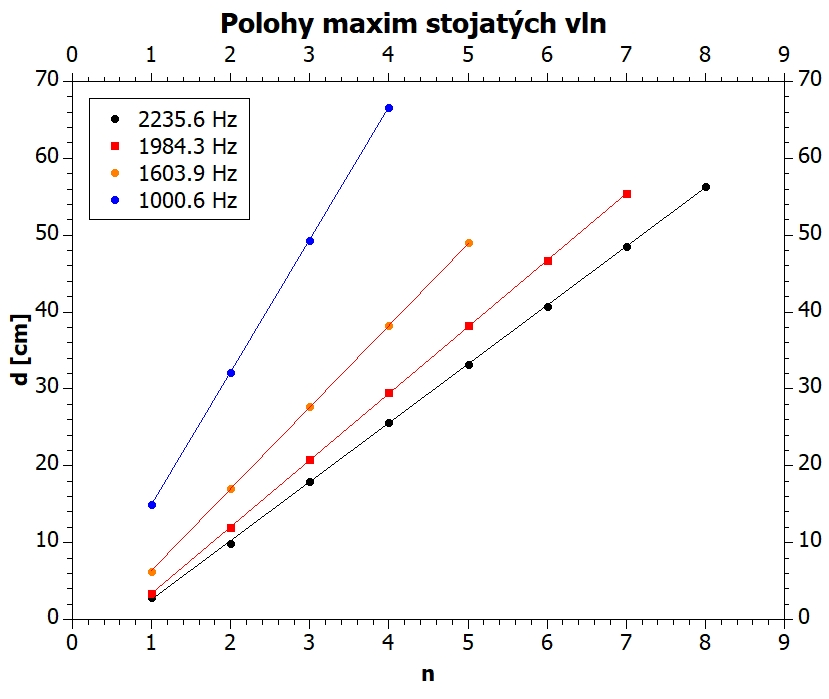
\includegraphics[width=0.6\linewidth, ]{max} 
	
\end{center}

Po aplikaci formule (5) a (7) získáme rychlosti zvuku a Poissonovy konstanty pro dané frekvence:

\begin{center}
	\begin{tabular}{|c|c|c|}
	\hline
	$f$ [Hz] & $c$ [$\rm m.s^{-1}$]& $\kappa$\\
	\hline
	2235.6 & 342.5 $\pm 3.7$& 1.386 $\pm 0.030$\\
	\hline
	1984.3 & 344.1 $\pm 3.5$& 1.399 $\pm 0.028$\\
	\hline
	1603.9 & 342.0 $\pm 3.5$&  1.382 $\pm 0.028$\\
	\hline
	1000.6 & 344.6 $\pm 3.5$& 1.404 $\pm 0.028$\\
	\hline
\end{tabular}
\end{center}
Tyto hodnoty jsme za použití hodnoty $\rho^{[1]} = 1.1748\,\rm g.cm^{-1} $ získali následujícím kódem:
\begin{verbatim}
p = ufloat (99398.8,0)
rho = ufloat (1.1748,0)
d1 = ufloat (17.22,0.03)
d2 = ufloat (10.66,0.02)
d3 = ufloat (8.67,0.01)
d4 = ufloat (7.66,0.03)
f1= ufloat (1000.6,10)
f2= ufloat (1603.9,16)
f3= ufloat (1984.3,19.84)
f4= ufloat (2235.6,22.35)
print ("c pro 1000 =", 2*d1*f1/100)
print ("c pro 1600 =", 2*d2*f2/100)
print ("c pro 1984 =", 2*d3*f3/100)
print ("c pro 2200 =", 2*d4*f4/100)



print ("k pro 1000 =", (2*d1*f1/100)**2 * rho /p)
print ("k pro 1600 =", (2*d2*f2/100)**2 * rho /p)
print ("k pro 1984 =", (2*d3*f3/100)**2 * rho/p)
print ("k pro 2200 =", (2*d4*f4/100)**2 * rho/p)
\end{verbatim}



	


	
	
	\section{Výsledek}
	
	Za použití Clément-Desormesovy metody nám hodnota Poissonovy konstanty po zaokrouhlení vyšla $\kappa = 1.37 \pm 0.06$ pro oba měřící přístroje. Při použití Kundtovy trubice nám Poissonova konstanta vyšla $\kappa_ {2235Hz}= 1.39 \pm 0.03, \kappa_ {1984Hz}= 1.40 \pm 0.03, \kappa_ {1604Hz}= 1.38 \pm 0.03, \kappa_ {1001Hz}= 1.40 \pm 0.03$.
	
	\section{Závěr}
	Jak lze z výsledků pozorovat, měření CD metodou se od skutečné hodnoty odchylovalo více. Jsem přesvědčen, že v této nepřesnosti hraje významnou roli ruční otevírání ventilu při adiabatické expanzi. Ve většině případů se mi nepodařilo ventil otevřít a následně zavřít dostatečně rychle, a tudíž došlo i~k~jiným dějům, které adiabatickou expanzi při otevírání a zavírání ventilu nahradily. U metody druhé jsem s výsledky spokojen, jelikož se skutečné hodnotě blížily mnohem více.
	\section{Zdroje}
[1] Air density calculator [on-line]\\ Dostupný z WWW: https://www.omnicalculator.com/physics/air-density
	
	% Nakonec nezapomeňte projet text programem vlna nebo vlnka, např.
	% 	vlna -m -l -n mojeuloha.tex
	% nebo zkontrolovat a opravit jednopísmenné předložky na koncích řádků ručně.
	
	
\end{document}
